\documentclass{article}
\usepackage[utf8]{inputenc}
\usepackage[toc,page]{appendix}
\usepackage{hhline}
\usepackage{hyperref}
\usepackage{amsmath}
\hypersetup{
    colorlinks=true,
    linkcolor = blue,
    urlcolor  = blue,
    citecolor = blue,
    anchorcolor = blue
}
\usepackage{minted}
\newcommand{\vect}[1]{\boldsymbol{\mathbf{#1}}}
\usepackage{subcaption}
\usepackage{graphicx}
\title{Extended Kalman Filters in Deep Learning}
\author{  Ananth Mahadevan\\
  \texttt{ananth.mahadevan@aalto.fi}
  \and
  Abhilash Jain\\
  \texttt{abhilash.jain@aalto.fi}}
\date{}

 \begin{document}

\maketitle
\clearpage
\tableofcontents
\clearpage 


\section{Introduction and Motivation }
\subsection{Problem Statement}
Since the beginning of the Deep Learning era, Stochastic Gradient Descent (SGD) based techniques, primarily through backpropagation of error gradients, have been the goto optimization techniques in any machine learning problem, and very few alternative avenues have been explored to see other techniques. In this Project we will explore one such optimization technique known as 'Extended Kalman Filters'\textbf{(EKF)} and try to understand its usage and its benefits over SGD-based techniques. This project will serve as a proof of concept that the EKF is a technique that can improve neural network accuracy and quality of training.
In the coming sections we will outline the work that has already been done in regards to this field. This will give an insight on how well researched the Kalman Filter techniques are and the utilization of them in existing systems. We then move on to give a brief summary on the data sets that we will consider in this project and their details. Later on we explain how we create our networks and train them using the techniques. Later we compare the results from the different methods and discuss them and their future scope.

\subsection{History}
We will give an introduction to Kalman Filters, it will not be mathematically intensive as most of our project focuses on it's extension. This section is meant to provide you leave with a general understanding of the theory and hopefully a sense of appreciation for the applications. There are many online sources for readers who are interested in a more detailed or mathematical approach such as \href{https://www.bzarg.com/p/how-a-kalman-filter-works-in-pictures/}{Kalman Filters with Pictuers}, or papers such as \href{http://byron.soe.ucsc.edu/projects/SeaSlug/Documents/Publications/Kalman\%20Filtering/An\%20Introduction\%20to\%20the\%20Kalman\%20Fiter2.pdf}{Introduction to Kalman Filters} \cite{Welch:1995:IKF:897831}.

Kalman filters have been around since the \textbf{1960s}, and it's not a new concept. It is in many ways what leads up to the neural network and AI revolution later in the 1980s. In essence, the Kalman filter is a set of equations that can recursively estimate the state of a \textbf{linear} dynamic system, in scenarios when the nature of the system itself is unknown and also accounts for all the statistical noise arising from measurements. It is able to do this by creating, predicting and update it's representation of the system state using matrices. It handles the noise that is bound to come from various sensory reading by assuming a distribution of the incoming noise and also incorporating this into it's calculation of the system's state. Through this process of \textbf{prediction} and \textbf{updating}, the Kalman filter is able to provide much more accurate estimates than those that will be made from only considering a single measurement could provide. 

The Kalman filter is critical to many \textbf{time series} and \textbf{signal processing} problems in real life. Many \textit{ballistic missile} systems, rocket guidance systems and many such \textbf{military targeting systems} utilize Kalman filters. Even systems as early as the \textbf{Apollo} missions utilized primitive Kalman filters to guide space missions. It is also an integral part of the Global Positioning System (GPS) to provide accurate real time measurements of location from satellite data.

\subsection{Need for EKF}
Given all the great and outstanding achievements that the previous section mentioned, the simple question arises \textit{Why Extended Kalman Filters}. This is a legitimate question, as most of the application of regular Kalman Filters described above have a critical flaw. They assume the system is \textbf{linear}. After taking the deep learning course, we can all agree that all problems are not linear in nature, in fact most physical systems and problems are \textbf{non-linear} in nature. 
\begin{equation}
\label{eqn:ekf}
\begin{aligned} \boldsymbol{x}_{k} &=f\left(\boldsymbol{x}_{k-1}, \boldsymbol{u}_{k}\right)+\boldsymbol{w}_{k} \\ \boldsymbol{z}_{k} &=h\left(\boldsymbol{x}_{k}\right)+\boldsymbol{v}_{k} \end{aligned}
\end{equation}
Here $\boldsymbol{x}_k$ is the state and $\boldsymbol{z}_k$ is the observation at time step $k$. $\boldsymbol{w}_k$ and $\boldsymbol{v}_k$ are the process and observation noises respectively. $\boldsymbol{u}_k$ is the control vector As we see here this formulation has the state evolving at each time step in accordance with a non-linear functions $f$ and $h$. This formulation leads to a modified set of equation called the Extended Kalman Filter. In relation with our project and deep learning, the non-linear function is the \textbf{neural network}. With this assumption we will model the weights of the neural network as the system state, $\boldsymbol{x}_k$ that we wish to estimate. 

A little bit of math to solidify the theory. Following the regular Kalman Filter, the extended version has 2 steps, predict and update. We will give a couple of equation that will be backbone of the EKF method that is implemented 

\subsubsection{Predict}
\begin{align}
    \textrm{Predicted state estimate}\qquad &\hat{\boldsymbol{x}}_{k | k-1}=f\left(\hat{\boldsymbol{x}}_{k-1 | k-1}, \boldsymbol{u}_{k}\right) \label{eqn:predict-state} \\	
    \textrm{Predicted covariance estimate} \qquad & \boldsymbol{P}_{k | k-1}=\boldsymbol{F}_{k} \boldsymbol{P}_{k-1 | k-1} \boldsymbol{F}_{k}^{\top}+\boldsymbol{Q}_{k} \label{eqn:predict-cov}
\end{align}
From Equation~\eqref{eqn:predict-state}, we see that predicting the state is just using the state at $k-1$ along with the control vector, this is essentially just predicting our updated weight matrix of a neural network. The covariance estimate of the state is the predicted system error and is calculated using the state transition matrix $\boldsymbol{F}_k$. In \eqref{eqn:predict-cov}, $\boldsymbol{Q}_k$ is the covariance of the process noise, i.e $\boldsymbol{w}_{k} \sim \mathcal{N}\left(0, \mathbf{Q}_{k}\right)$.
$\boldsymbol{R}_k$ is the Observation Noise.
\subsubsection{Update}

\begin{align}
    \textrm{Innovation or measurement residual	}\qquad & \tilde{\boldsymbol{y}}_{k}=\boldsymbol{z}_{k}-h\left(\hat{\boldsymbol{x}}_{k | k-1}\right) \label{eqn:update-innovation} \\
    \textrm{Innovation (or residual) covariance	} \qquad & \boldsymbol{S}_{k}=\boldsymbol{H}_{k} \boldsymbol{P}_{k | k-1} \boldsymbol{H}_{k}^{\top}+\boldsymbol{R}_{k} \label{eqn:update-inno-cov}\\
    \textrm{Near-optimal Kalman gain}\qquad & \boldsymbol{K}_{k}=\boldsymbol{P}_{k | k-1} \boldsymbol{H}_{k}^{\top} \boldsymbol{S}_{k}^{-1} \label{eqn:kalman-gain}\\
    \textrm{Updated state estimate	}\qquad &\hat{\boldsymbol{x}}_{k | k}=\hat{\boldsymbol{x}}_{k | k-1}+\boldsymbol{K}_{k} \tilde{\boldsymbol{y}}_{k} \label{eqn:update-state} \\
    \textrm{Updated covariance estimate} \qquad & \boldsymbol{P}_{k | k}=\left(\boldsymbol{I}-\boldsymbol{K}_{k} \boldsymbol{H}_{k}\right) \boldsymbol{P}_{k | k-1} \label{eqn:update-cov}
\end{align}
These update statements start from an observation $\boldsymbol{z}_k$, in our case the true label(or value) of an input, and calculate the residual as in Equation~\eqref{eqn:update-innovation}. Here the function $h$, is our neural network and $h(\hat{\boldsymbol{x}}_{k | k-1})$ is the output of our network Then we measure the covaraince of the expected innovation in \eqref{eqn:update-inno-cov}. Here the most important factor for us is the state observation matrix $\boldsymbol{H}_k$, it is defined as 
\[ 
\boldsymbol{H}_{k}=\left.\frac{\partial h}{\partial \boldsymbol{x}}\right|_{\hat{\boldsymbol{x}}_{k | k-1}}
\]
This is the matrix that contains the gradients of network weights( or parameters). This is the reason why EKF has some ground to replace the stochastic gradent descent methods, as their roots are in the same gradients of the network. EKF here uses this in turn to update the covariance of the error and also the gain of the Kalman Filter as seen in \eqref{eqn:kalman-gain}. We then update our state, i.e. weights of the network, which act as an optimizer step in gradient descent. This is seen in \eqref{eqn:update-state}, where we utilize the residue $\tilde{\boldsymbol{y}}_k$ and the gain $\boldsymbol{K}_k$.We also update the estimate of the system covariance $\boldsymbol{P}_{k|k}$.
\\ \\
Although these seem very complicated set of matrices and equation, you can clearly see in our implementation in Appendix of \texttt{knn.py},line number~\ref{code:ekf}, it is pretty much a direct implementation of the equations mentioned, in \texttt{numpy} matrix multiplications. The $\boldsymbol{H}_k$, is calculated using the derivative of the activation function of the neurons, in a way very similar to \texttt{pytorch}'s implementation. 

\clearpage
\section{Data description}
We be using 3 datasets from the UCI machine learning repositiory \cite{Dua:2019}. They are namely the Abalone, Bike sharing \cite{Bikes} and Wine quality \cite{Winequality}. These are similar to the datasets used in \cite{Chernodub2014} and \cite{Main_EKS_Paper}. 

We will now provide a short description of the datasets and then an overall view of the data

\subsection{Abalone Dataset}
This is a dataset where the task is to predict the age of an abalone, which is a kind of marine snail. Their meat is used a culinary item and their shells for \textit{mother of pearl} for jewelery .The data is the hysical measurements of an abalone.The true age of abalone is determined by cutting the shell through the cone, staining it, and counting the number of rings through a microscope. This is a time-consuming task. 

There are other measurements, which are easier to obtain, can be used to predict the age. These are the attributes that the dataset contains as shown in Table~\ref{tab:Abalone}

\begin{table}[ht]
    \centering
    \begin{tabular}{c|c|c|l}
    \hline
    Name	&	Data Type &	Measurement	& Description\\
    \hhline{=|=|=|=}
	Sex		&categorical	&		M, F, and I (infant)\\
	Length		&continuous	&mm	&Longest shell measurement\\
	Diameter	&continuous	&mm	&perpendicular to length\\
	Height		&continuous	&mm	&with meat in shell\\
	Whole weight	&continuous	&grams	&whole abalone\\
	Shucked weight	&continuous	&grams	&weight of meat\\
	Viscera weight	&continuous	&grams	&gut weight (after bleeding)\\
	Shell weight	&continuous	&grams	&after being dried\\
	Rings		&integer			&&+1.5 gives the age in years\\
	\hline
    \end{tabular}
    \caption{Abalone Dataset Description}
    \label{tab:Abalone}
\end{table}
As seen the last attribute, the rings is the quantity that we wish to predict. All the data is in continuous range, except the sex of the abalone. This will be converted into a categorical data type when pre-processing.
\subsection{Bike Sharing Dataset}
This dataset has the hourly count of rental bikes for 2011 and 2012 along with the corresponding seasonal and weather data. It is a regression task where we must predict the number of bikes that will be rented in any hour given the weather conditions and details of the day in question. There are many studies that have shown the rental bike count is highly correlated with the environmental and seasonal settings. Also as the given dataset has some time related information, it will be a good measure of the performance of the EKF, which is already known to be good for timeseries data. This dataset also has upwards of 17000 data points that will also test the EKF method as it will have a larger number of samples to propagate at every epoch.  


The attributes of the dataset are as follows

\begin{enumerate}
    \item instant: record index
	\item dteday : date
    \item season : season 
        \begin{itemize}
            \item[-] 1: Spring
            \item[-] 2: Summer
            \item[-] 3: Fall 
            \item[-] 4: Winter 
        \end{itemize}
    \item yr : year (0: 2011, 1:2012)
	\item mnth : month ( 1 to 12)
	\item hr : hour (0 to 23)
	\item holiday : weather day is holiday or not 
	\item weekday : day of the week
	\item workingday : if day is neither weekend nor holiday is 1, otherwise is 0.
	\item weathersit : weather situation
	\begin{itemize}
		\item[-] 1: Clear, Few clouds, Partly cloudy, Partly cloudy
		\item[-] 2: Mist + Cloudy, Mist + Broken clouds, Mist + Few clouds, Mist
		\item[-] 3: Light Snow, Light Rain + Thunderstorm + Scattered clouds, Light Rain + Scattered clouds
		\item[-] 4: Heavy Rain + Ice Pallets + Thunderstorm + Mist, Snow + Fog
	\end{itemize}
	\item temp : Normalized temperature in Celsius. The values are divided to 41 (max)
	\item atemp: Normalized feeling temperature in Celsius. The values are divided to 50 (max)
	\item hum: Normalized humidity. The values are divided to 100 (max)
	\item windspeed: Normalized wind speed. The values are divided to 67 (max)
	\item casual: count of casual users
	\item registered: count of registered users
	\item cnt: count of total rental bikes including both casual and registered
\end{enumerate}
We need to predict the last attribute \textit{cnt} or the total count of the number of rental bikes. 

\subsection{Wine quality Dataset}
This dataset contains the physiochemical, i.e. the physical and chemical attributes of almost 5000 different typed of white wine. Each of these data points are assigned a quality number which is what we aim to predict. This data is a regular run of the mill classification/regression task. 
\begin{enumerate}
   \item fixed acidity
   \item volatile acidity
   \item citric acid
   \item residual sugar
   \item chlorides
   \item free sulfur dioxide
   \item total sulfur dioxide
   \item density
   \item pH
   \item sulphates
   \item alcohol
   \item quality: (score between 0 and 10)
\end{enumerate}

We actually do not require any domain knowledge for each individual dataset as the way we have framed the problem is to explore and investigate the performance of the \textit{Extended Kalman Filter} as an alternative to the regular stochastic gradient descent. Hence the algorihtm ought to work well given any dataset for a given neural network. Hence the overview of the datasets considered are given in Table~\ref{tab:datasets}.  
\begin{table}[ht]
    \centering
    \begin{tabular}{cccccc}
        \hline
         Dataset &  Size & Training & Testing & Validation & Dimensionality\\ \hhline{======}
         Abalone & 4177 &2089 &1044 &1044 &8 \\
         Bike Sharing & 17,379 & 8989 & 4345 & 4345 & 16\\
         Wine Quality & 4898 & 2449 &1225& 1224 & 11\\
         \hline
    \end{tabular}
    \caption{Data-sets and attributes}
    \label{tab:datasets}
\end{table}

\clearpage
\section{Method}

We conduct different experiments(regression tasks) across different model definitions. We choose basic Neural Network architectures as a starting point to prove the efficacy of the EKF-based architectures and slightly more complex Neural Networks for SGD-based approaches.\\
\\
The current models are built with SGD in mind and finding/building Complex models with EKF-based architectures would be the next steps of this project, when there is enough proof presented that Simple EKF-based architectures are better than the SGD-based counterparts present today.\\
The models we experiment with in the project are novel in the sense that 1) there are very few benchmarking done within this domain such that we just pick up models. 2)  they not only out-perform their SGD counter-parts but also the better/complex SGD-based architectures\\
\\
\subsection{EKF}
The neural network model for the EKF trained network is a simple one. A single hiddel layer with 10 neurons, which have an one of the 3 chosen activation functions: \textbf{sigmoid}, \textbf{tanh} and \textbf{ReLu}. The implementation is kept this simple as it allows the constriction of the network weights as simple \texttt{numpy} matrices and back propagation of gradients as a simple matrix multiplications utilizing the derivative of the activations functions mentioned. This is very similar to how the pytorch's \texttt{Autograd} network works. We opted a pure \texttt{numpy} implementation as it speeds up computations and is faster than switching between \texttt{pytorch tensors} and \texttt{numpy ndarrays}. The EKF learning is also then a simple set of matrix equations involving the previously discussed $\boldsymbol{P}$, $\boldsymbol{Q}$, $\boldsymbol{R}$ and the weight matrix $W$. A quick refernce to this part of the code is found at Line~\ref{code:ekf}.

The simplicity of the EKF model allows us to showcase how few layers and neurons are needed for the Kalman Filter to effectively find optimal network weights for the same data compared to SDG, discussed next.
\subsection{SGD}
To effectively compare and display the capability of the EKF we have opted to perform tests on 3 architectures ustilizing SGD
\begin{itemize}
    \item \textbf{1 Hidden Layer}:\\
    This is the same network architecture as the one used to train the EKF model, hence this provides a \textbf{direct comparison} between the ability for SGD to train a NN with one hidden layer with  10 neurons.
    \item \textbf{2 Hidden layers}:\\
    This NN has a 10x10 architecture, meaning two hidden layers and 10 neurons in each layer. This is a more complex model than the baseline EKF architecture.
    \item \textbf{3 Hidden Layers}:\\
    This will have a 10x10x10 architecture, 10 neurons in each of the threee hidden layers.
\end{itemize}
All the above models will be implemented in \texttt{pytroch}, due to the ease of model creation and trainig using \texttt{Adam} as an optimizer and also was tested with each of the activation functions mentioned above. 

Our Data-set is split into Training, Testing and Validation Data-sets as mentioned in the earlier section. The more complex SGD netowrks have the drawback of overfitting to the training dataset. Hence we apply \textbf{Early Stopping}
on hold out validation set such that the SGD-based. In the results section we discuss how early stopping and network complexity affects EKF and SGD based techniques.

\clearpage
\section{Experiments and results}
We will describe here the results that we obtained from training out neural networks using both the \textit{Extended Kalman Filter} and \textit{Stochastic Gradient Descent}.

\subsection{Role of \textbf{Q} and \textbf{R} }
We have 3 parameters to the EKF training module, these are initial values of the matrices $\boldsymbol{P}$, $\boldsymbol{Q}$ and $\boldsymbol{R}$, which are the weight covaraince, process covaraince and data covarainces respectively. As mentioned in \cite{Main_EKS_Paper} the initial values $\boldsymbol{P}$ are not significant as they are rarely known at the beginning of training, and whatever $\boldsymbol{P}_0$ is, it is quickly adjusted by the Kalman Gain matrix $\boldsymbol{K}$.

The Kalman gain matrix that affects the weght update has this dependency
\[ \boldsymbol{K}_k \propto \frac{\boldsymbol{Q}_k}{\boldsymbol{R}_k}\]
This is seen by changing the values of  $\boldsymbol{Q}$ and $\boldsymbol{R}$ and checking the effect on the validation error. We see that in Fig~\ref{fig:Q} , the highest value of noise corresponds to the highest value of $\boldsymbol{Q}$ has the highest level of noise. Hence directly seen that the higher that $\boldsymbol{Q}_k$ is, higher the gain $\boldsymbol{K}_k$ is , which affects the state update of $\boldsymbol{x}_k$. Hence a smaller value of $\boldsymbol{Q}$ gives a smoothing behaviour to the error in each epoch.
\begin{figure}[ht]
    \centering
    \begin{subfigure}[b]{0.5\linewidth}
        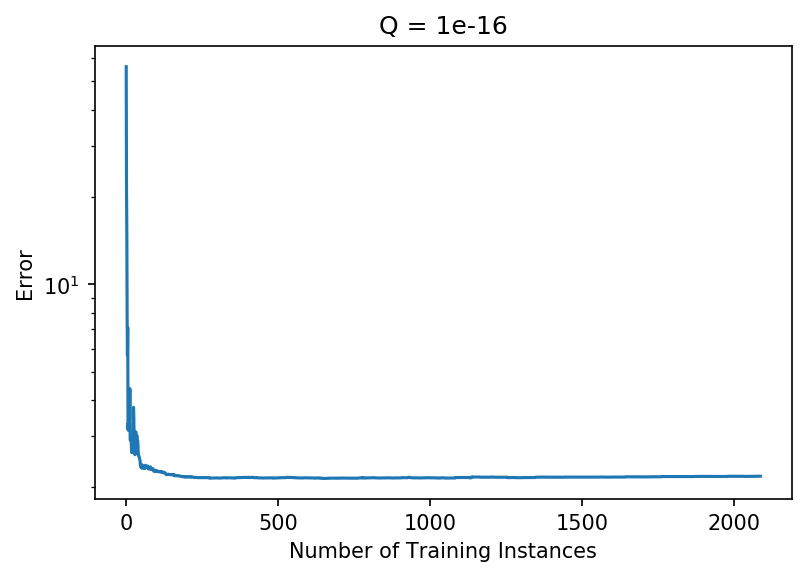
\includegraphics[width=\linewidth]{Q1e-16.png}
        \caption{}
        \label{fig:Q1e-16}
    \end{subfigure}%
    \begin{subfigure}[b]{0.5\linewidth}
        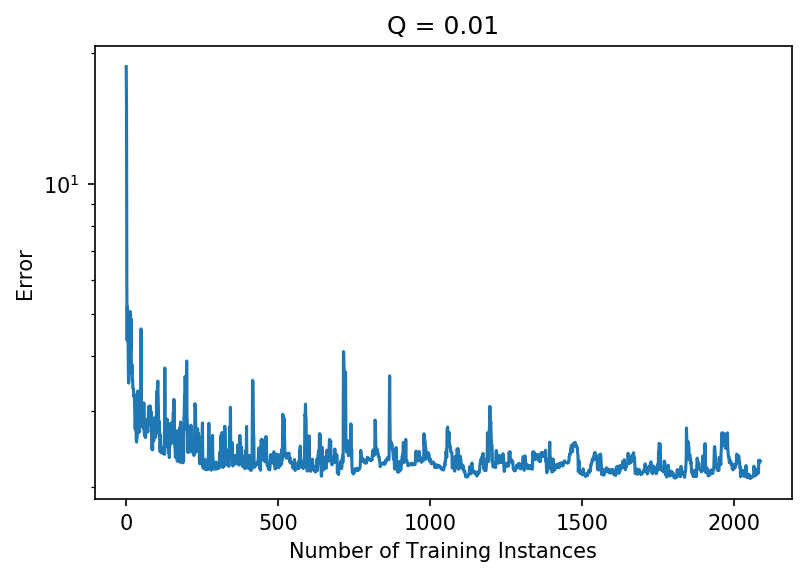
\includegraphics[width=\textwidth]{Q001.png}
        \caption{}
        \label{fig:Q1e-2}
    \end{subfigure}%
    
    \begin{subfigure}[b]{0.5\linewidth}
        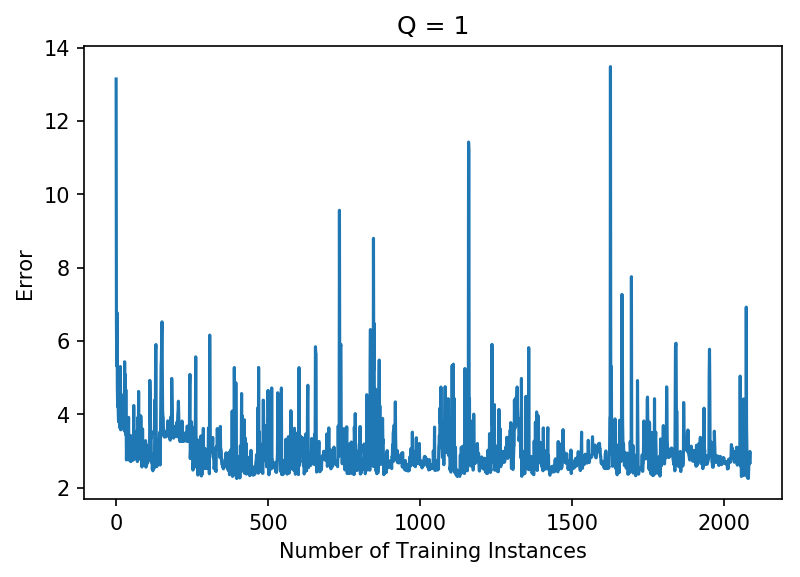
\includegraphics[width=\textwidth]{Q1.png}
        \caption{}
        \label{fig:Q1}
    \end{subfigure}%
    \caption{Effect of $\boldsymbol{Q}$ on the error after each sample in an epoch for the Abalone dataset, (a) $\boldsymbol{Q}=1e-16$, (b) $\boldsymbol{Q}=0.01$, (c) $\boldsymbol{Q}=1$}
    \label{fig:Q}
\end{figure}

Figure~\ref{fig:R} was creating using the Bike sharing dataset, as it has a larger number of samples per epoch. In this we see that the larger $\boldsymbol{R}$ is the smoother the reduction in the validation error is. The smaller $\boldsymbol{R}$ is the more noise is present in the estimation errors, even causing random spikes as seen in \ref{fig:R1e-2}. The value of $\boldsymbol{R}$, can be thought of as an inverse of the learning rate of the neural network. 
\begin{figure}[ht]
    \centering
    \begin{subfigure}[b]{0.45\linewidth}
        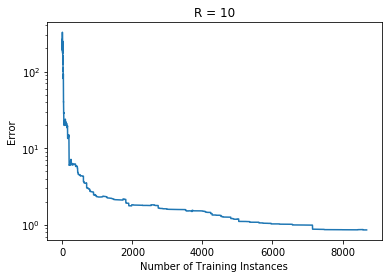
\includegraphics[width=\linewidth]{R_10.png}
        \caption{}
        \label{fig:R10}
    \end{subfigure}%
    \begin{subfigure}[b]{0.45\linewidth}
        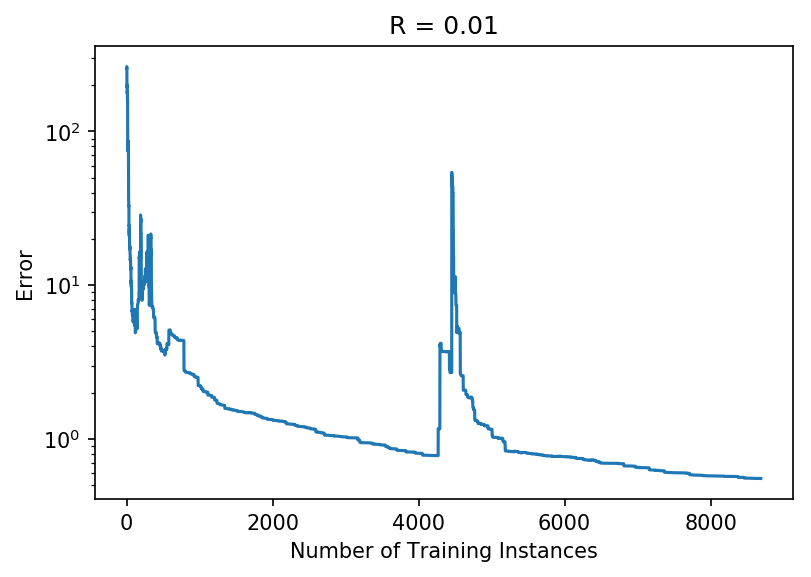
\includegraphics[width=\textwidth]{R_001.png}
        \caption{}
        \label{fig:R1e-2}
    \end{subfigure}%
    
    \begin{subfigure}[b]{0.5\linewidth}
        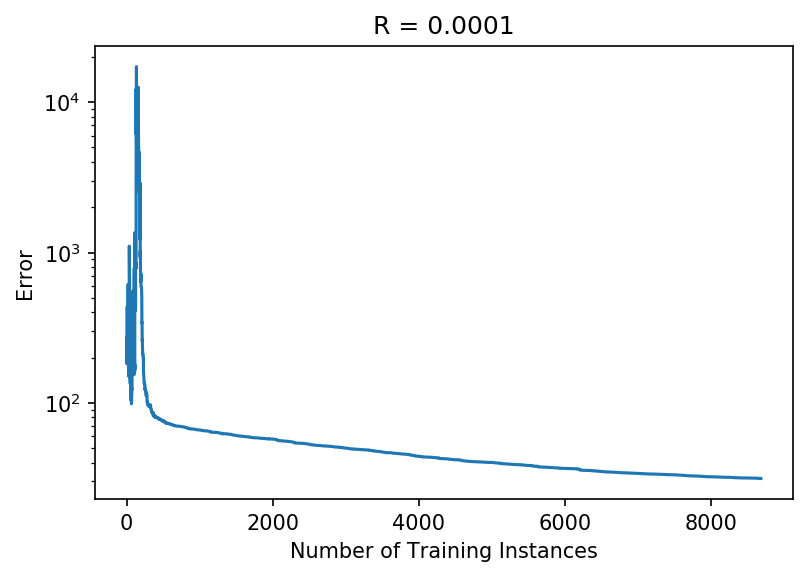
\includegraphics[width=\textwidth]{R1e-4.png}
        \caption{}
        \label{fig:R1e-4}
    \end{subfigure}%
    \caption{Effect of $\boldsymbol{R}$ on the error after each sample in an epoch for the Bike haring dataset, (a) $\boldsymbol{R}=10$, (b) $\boldsymbol{R}=0.01$, (c) $\boldsymbol{R}=1e-4$}
    \label{fig:R}
\end{figure}

\subsection{Training Statistics}
A major question to ask is how fast is EKF when compared to SGD. This is a tough question to answer as it is an 'Apples to oranges comparison'. It is true that SGD takes much less time to run 20 epochs of the same 10 neuron model than it takes EKF. This is mainly due to the fact that EKF involves more matrix multiplications that are time consuming operations compared to gradient descent algorithms. But the key question to ask is, \textit{at the end of 20 epochs, which methods has a better test error?}. 


This tends to showcase the differences between the two approaches. As seen in Figure~\ref{fig:validation}, both the graphs show the error on the validation set for the Bike Sharing dataset, for a 10 neuron network. Both EKF and SGD both start at a very high error of 250, but within one epoch, EKF already achieves the same error as SGD does only around epoch 4000. We choose to highlight this fact, as most traditional application of EKF are in online learning, when the data is seen as it arrives. Hence, we could technically run EKF for one epoch and get very good results, compared to the need for 1000s of epochs for gradient descent.  
\begin{figure}[h!]
    \centering
    \begin{subfigure}[b]{0.45\linewidth}
        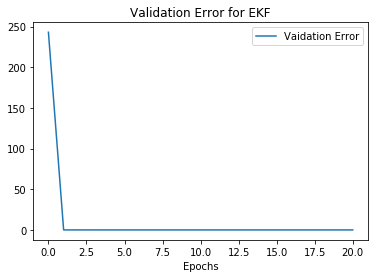
\includegraphics[width=\linewidth]{EKF_validation.png}
        \caption{EKF}
        \label{fig:ekf-validation}
    \end{subfigure}
    \begin{subfigure}[b]{0.45\linewidth}
        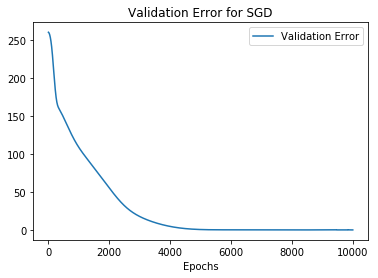
\includegraphics[width=\linewidth]{SGD_validation.png}
        \caption{SGD}
        \label{fig:sgd-validation}
    \end{subfigure}
    \caption{Graphs of validation error vs epochs for a 10 neuron network for the Bike Sharing dataset.(a) When trained with EKF for 20 epochs.(b) When trained with SGD for 10,000 epochs}
    \label{fig:validation}
\end{figure}

The next question that is usually asked is that, \textit{why only a single hidden layer of 10 neurons?}. The argument being that, SGD will produce better error rates and predictions with more hidden layers, see Figre~ \ref{fig:stack}, and more neurons per hidden layer. This though maybe true for much more complex domain problems such as computer vision and language modelling. We see in our project that adding more layers only produces minor gains in validation error, but also at the same time take longer to run. Due to this fact, we compare our EKF results with one hidden layer of 10 neurons with up to 3 hidden layers with 10 neurons in each layer. Results clearly indicate that still EKF has better performance than multilayer networks. There are possible implementation for multi-layer hidden networks with EKF as seen in \cite{Evol}. These unfortnately are out of the scope of the project and will be discussed briefly in future works section.
\begin{figure}[ht]
    \centering
    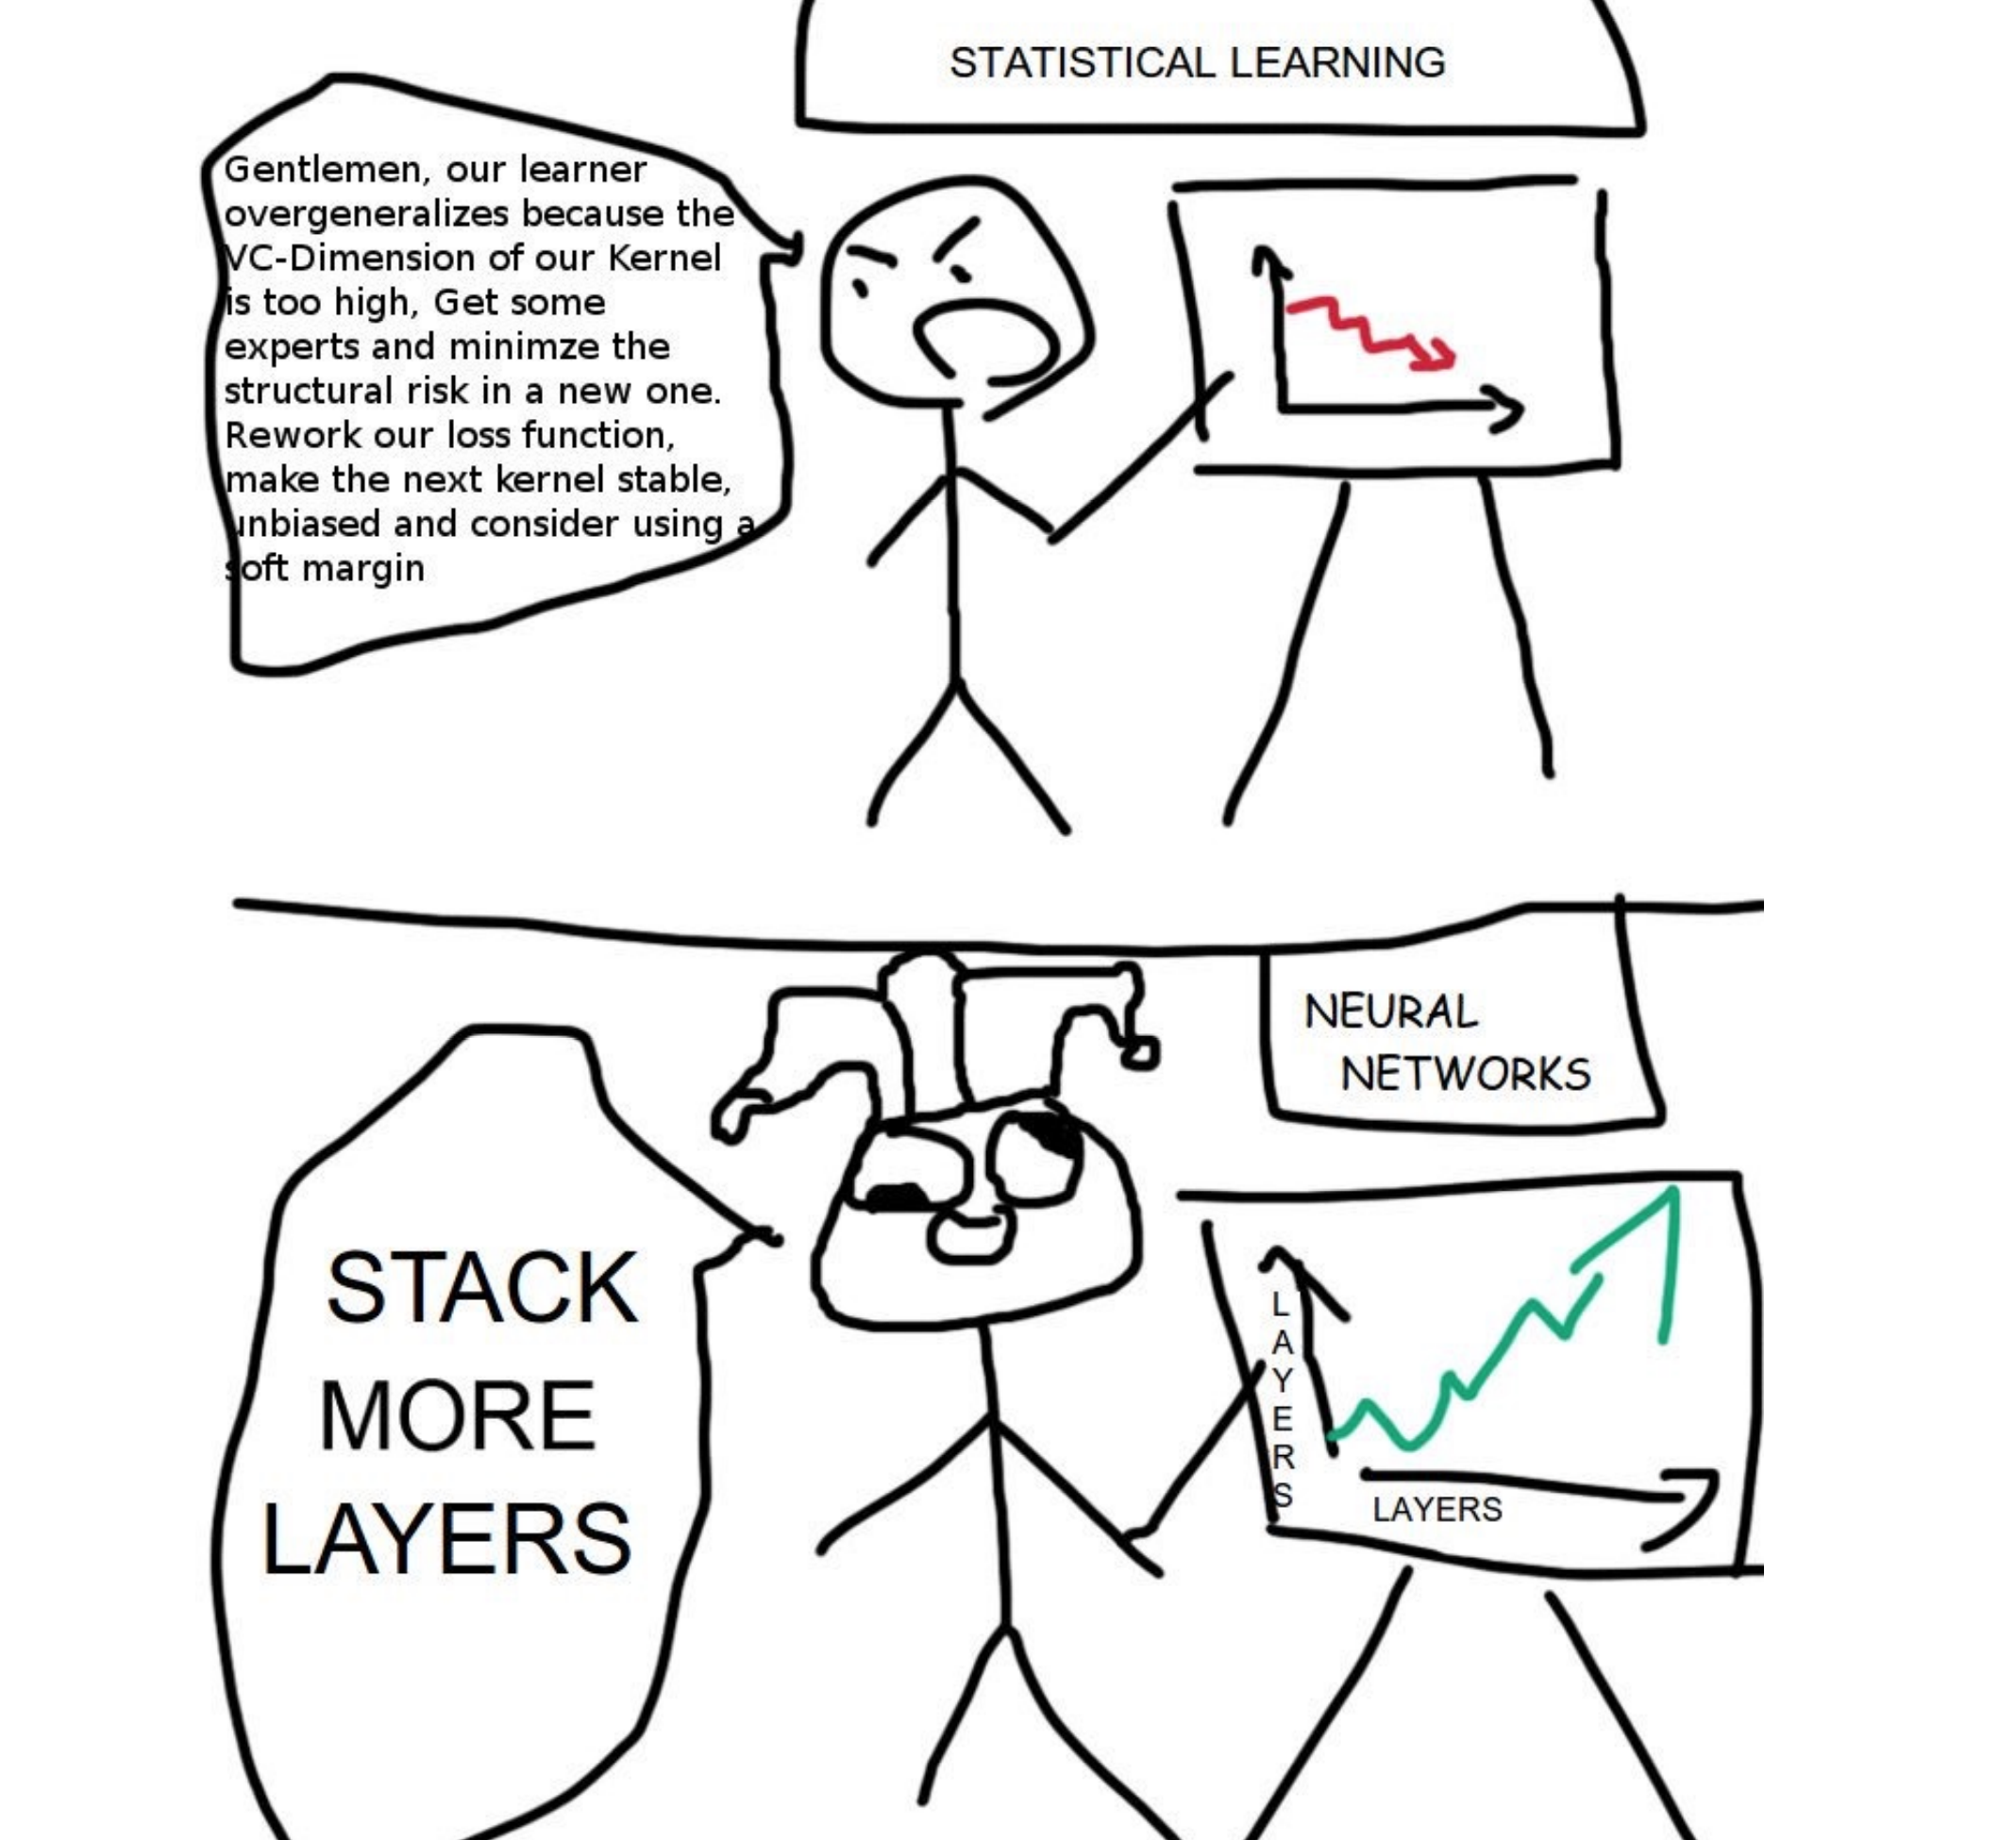
\includegraphics[width=0.5\linewidth]{stack.png}
    \caption{Funny Neural Network meme}
    \label{fig:stack}
\end{figure}
\clearpage
\subsection{Comparitive Results}
The training were performed on a computer with the following specifications:
\begin{itemize}
    \item Cpu: 19-8950HK
    \item RAM: 32 GBs
    \item GPU: GTX-1050ti Max Q
\end{itemize}
The average running times are shown in 
\begin{table}[ht]
    \centering
    \begin{tabular}{lrrrrr}
        \hline
         Dataset & EKF  & SGD 10 & SGD 10x10 & SGD 10x10x10 \\
         \hhline{======}
         Abalone & 7s & 25s & 40s & 47s \\
         Bike Sharing & 49s & 55s & 1min 10s & 1min 25s \\
         Wine Quality & 11s & 35s & 40s & 50s\\
    \end{tabular}
    \caption{Average running times for \textbf{20} epcohs of EKF and \textbf{10,000} epochs of SGD for different datasets with different number of layers, i.e 10, 10x10 and 10x10x10}
    \label{tab:my_label}
\end{table}

The results in Table~\ref{tab:results} show the lowest training error achieved in 10 runs of the data set with the non-linear activation mentioned inside the bracket. Each data set was trained using either EKF for 20 epochs or SGD for architectures having one hidden layer with 10 neurons, i.e. \textit{SGD 10}, 2 hidden layers with 10 neurons each, i.e. \textit{SGD 10x10}, or  with 3 hidden layers each with 10 neurons, i.e. \textit{SGD 10x10x10}. As mentioned in the previous sections, the disadvantage of running gradient descent with deeper networks is that they tend to start \textbf{overfitting} very soon, leding to performance degradation. This is why we also mention the lowest vlidation error achieved at which epoch (rounded down to the nearest 1000) inside the brackets of each results. 
\begin{table}[ht]
    \centering
    \begin{tabular}{lrrrrr}
        \hline
         Dataset & EKF  & SGD 10 & SGD 10x10 & SGD 10x10x10 \\
         \hhline{======}
         Abalone (sigmoid)& 1.983(20) & 2.011(10,000)& 1.995(6000) &1.973(5000) \\
         Abalone (tanh)& 2.029(20) & 2.057(10,000) & 1.981(6000) & 2.009(2000) \\
         Abalone (ReLu)& 2.082(20) & 2.094(10,000)& 2.043(4000) &2.032(2000)  \\
         \hline
         Bike Sharing (sigmoid)& 23.916(20) &62.323(10,000)&63.513(10,000) & 180.173(10,000) \\
         Bike Sharing (tanh)&21.999(20) &60.813(10,000) & 60.812(10,000) & 66.042(10,000) \\
         Bike Sharing (ReLu)&  0.00038(20) & 0.255(10,000) & 0.058(4000) &0.115 (5000)\\
         \hline
         Wine Quality (sigmoid)& 0.6984(20) &0.7015 (9000) & 0.7068 (6000) & 0.7025 (4000)\\
         Wine Quality (tanh)& 0.6933(20) &  0.6948(10,000) & 0.6982(5000) & 0.7004(3000)\\
         Wine Quality (ReLu)& 0.7073(20)& 0.7274(10,000) & 0.7492 (5000) & 0.7372(6000)\\
         \hline
\\
    \end{tabular}
    \caption{Mean validation error for all datasets with different activation functions, when trained with EKF or SGD with different architectures. EKF was always trained for 20 epochs. SGD was trained for different number of hidden layers, with the lowest validation error reported along with the early stopping epoch it was achieved at }
    \label{tab:results}
\end{table}

Analyzing the resuts from Table~\ref{tab:results}, it is clear that in all databases and most activation functions the EKF training methods achieve much better validation errors than their SGD counter parts trained for much more epochs.
\clearpage
\section{Conclusion }
In terms of Speed and Error, EKF clearly outperforms SGD in very low amounts of epoch. We can see that the error was reduced considerably when we use the ReLu activation.
\subsection{Benefits}
\subsection{Disadvantages}
Current Drawback of EKF is that this cannot be implemented in Deep Neural Networks,\cite{Evol} Although very recent work has proved that these can be implemented, but again no open implementation exists and is quite difficult to change the architecture as the paper suggest
\subsection{Future Work}
To truly harness the power of EKF, we need to invest considerable amount of research to implement these in more and more complex architectures currently present in the Deep Learning World. \cite{Evol} is a really good starting point and more tasks and different kind of data can be used 
\clearpage
\appendix
\appendixpage
\section{Code}
The following sections will contain certain part of the code. The results and reproducability are on Jupyter notebooks and can be viewed at the github link \url{https://github.com/ananth1996/Neural-Netowork-Extended-Kalman-Filter}. The  \href{https://github.com/ananth1996/Neural-Netowork-Extended-Kalman-Filter/blob/master/Evaluation.ipynb}{Evaluation Notebook} is available at the link, and we strongly encourage you to grade us based on the complete code available on the GitHub repository.
\subsection{knn.py}
This is the file that contains the class definition for the 
\begin{minted}[breaklines, escapeinside=||]{python}
"""
Contains a class for EKF-training a feedforward neural-network.
This is primarily to demonstrate the advantages of EKF-training.
See the class docstrings for more details.
This module also includes a function for loading stored KNN objects.

"""
from __future__ import division
import numpy as np; npl = np.linalg
from scipy.linalg import block_diag
from time import time
import pickle
from tqdm import tqdm_notebook as tqdm

##########

def load_knn(filename):
    """
    Loads a stored KNN object saved with the string filename.
    Returns the loaded object.

    """
    if not isinstance(filename, str):
        raise ValueError("The filename must be a string.")
    if filename[-4:] != '.knn':
        filename = filename + '.knn'
    with open(filename, 'rb') as input:
        W, neuron, P = pickle.load(input)
    obj = KNN(W[0].shape[1]-1, W[1].shape[0], W[0].shape[0], neuron)
    obj.W, obj.P = W, P
    return obj

##########

class KNN:
    """
    Class for a feedforward neural network (NN). Currently only handles 1 hidden-layer,
    is always fully-connected, and uses the same activation function type for every neuron.
    The NN can be trained by extended kalman filter (EKF) or stochastic gradient descent (SGD).
    Use the train function to train the NN, the feedforward function to compute the NN output,
    and the classify function to round a feedforward to the nearest class values. A save function
    is also provided to store a KNN object in the working directory.

    """
    def __init__(self, nu, ny, nl, neuron, sprW=5):
        """
            nu: dimensionality of input; positive integer
            ny: dimensionality of output; positive integer
            nl: number of hidden-layer neurons; positive integer
        neuron: activation function type; 'logistic', 'tanh', or 'relu'
          sprW: spread of initial randomly sampled synapse weights; float scalar

        """
        # Function dimensionalities
        self.nu = int(nu)
        self.ny = int(ny)
        self.nl = int(nl)

        # Neuron type
        if neuron == 'logistic':
            self.sig = lambda V: (1 + np.exp(-V))**-1
            self.dsig = lambda sigV: sigV * (1 - sigV)
        elif neuron == 'tanh':
            self.sig = lambda V: np.tanh(V)
            self.dsig = lambda sigV: 1 - sigV**2
        elif neuron == 'relu':
            self.sig = lambda V: np.clip(V, 0, np.inf)
            self.dsig = lambda sigV: np.float64(sigV > 0)
        else:
            raise ValueError("The neuron argument must be 'logistic', 'tanh', or 'relu'.")
        self.neuron = neuron

        # Initial synapse weight matrices
        sprW = np.float64(sprW)
        self.W = [sprW*(2*np.random.sample((nl, nu+1))-1),
                  sprW*(2*np.random.sample((ny, nl+1))-1)]
        self.nW = sum(map(np.size, self.W))
        self.P = None

        # Function for pushing signals through a synapse with bias
        self._affine_dot = lambda W, V: np.dot(np.atleast_1d(V), W[:, :-1].T) + W[:, -1]

        # Function for computing the RMS error of the current fit to some data set
        self.compute_rms = lambda U, Y: np.sqrt(np.mean(np.square(Y - self.feedforward(U))))

####

    def save(self, filename):
        """
        Saves the current NN to a file with the given string filename.

        """
        if not isinstance(filename, str):
            raise ValueError("The filename must be a string.")
        if filename[-4:] != '.knn':
            filename = filename + '.knn'
        with open(filename, 'wb') as output:
            pickle.dump((self.W, self.neuron, self.P), output, pickle.HIGHEST_PROTOCOL)

####

    def feedforward(self, U, get_l=False):
        """
        Feeds forward an (m by nu) array of inputs U through the NN.
        Returns the associated (m by ny) output matrix, and optionally
        the intermediate activations l.

        """
        U = np.float64(U)
        if U.ndim == 1 and len(U) > self.nu: U = U[:, np.newaxis]
        l = self.sig(self._affine_dot(self.W[0], U))
        h = self._affine_dot(self.W[1], l)
        if get_l: return h, l
        return h

####

    def classify(self, U, high, low=0):
        """
        Feeds forward an (m by nu) array of inputs U through the NN.
        For each associated output, the closest integer between high
        and low is returned as a (m by ny) classification matrix.
        Basically, your training data should be (u, int_between_high_low).

        """
        return np.int64(np.clip(np.round(self.feedforward(U), 0), low, high))

####

    def train(self, nepochs, U, Y, U_val, Y_val, method, P=None, Q=None, R=None, step=1, tolerance=-1, patience=1, print_every=1):
        """Function to train the neural network
        
        Arguments:
            nepochs {int} -- the total number of epochs the network should be trained for
            U {numpy array} -- Input training data, shape (m,nu), m samples and nu dimensions
            Y {numpy aray} -- Output training labels, shape (m,ny)
            U_val {numpy array} -- Validation input data
            Y_val {numpy array} -- Validation label
            method {str} -- extended kalman filter 'ekf' or stochastic gradient descent 'sgd
        
        Keyword Arguments:
            P {float or numpy array} -- Initial weight covaraince matrix, if float then diagonal matrix, else positive defintite matrix of shape (nW,nW) (default: {None})
            Q {float or numpy array} -- Initial process covariance matrix, if float then diagonal matrix, else semi positive defintie matrix of shape (nW,nW) (default: {None})
            R {float or numpy array } -- Initial Data Covaraince for ekf, if float then diagnoal matrix, else positive definite matrix of shape (ny,ny)  (default: {None})
            step {int} -- ste=-size scaling (default: {1})
            tolerance {int} -- tolerance limit for early stopping (default: {-1})
            patience {int} -- number of epochs to be patient for in early stopping (default: {1})
            print_every {int} -- for old display logic (default: {1})
        
        Raises:
            ValueError: if size of U and Y are different 
            ValueError: if shape of U is wrong
            ValueError: if shape of Y is wrong
            ValueError: if P is None and self.P is not specified
            ValueError: if P is not a float or a matrix of shape (nW,nW)
            ValueError: if Q is not a float or a matrix of shape (nW,nW)
            ValueError: if R is not specified for training
            ValueError: if R is not a float or a matrix of shape (ny,ny)
            ValueError: if R matrix is not positive definite 
            ValueError: if training method is not efk or sgd
        
        Returns:
            RMS -- List of validation RMS errors 
            epoch_errors -- The validation errors in the first epoch after each sample  
         """

        # Verify data
        U = np.float64(U)
        Y = np.float64(Y)
        if len(U) != len(Y):
            raise ValueError("Number of input data points must match number of output data points.")
        if (U.ndim == 1 and self.nu != 1) or (U.ndim != 1 and U.shape[-1] != self.nu):
            raise ValueError("Shape of U must be (m by nu).")
        if (Y.ndim == 1 and self.ny != 1) or (Y.ndim != 1 and Y.shape[-1] != self.ny):
            raise ValueError("Shape of Y must be (m by ny).")
        if Y.ndim == 1 and len(Y) > self.ny: Y = Y[:, np.newaxis]
        if Y_val.ndim == 1 and len(Y_val) > self.ny: Y_val = Y_val[:, np.newaxis]

        # Set-up
        if method == 'ekf':
            self.update = self._ekf

            if P is None:
                if self.P is None:
                    raise ValueError("Initial P not specified.")
            elif np.isscalar(P):
                self.P = P*np.eye(self.nW)
            else:
                if np.shape(P) != (self.nW, self.nW):
                    raise ValueError("P must be a float scalar or (nW by nW) array.")
                self.P = np.float64(P)

            if Q is None:
                self.Q = np.zeros((self.nW, self.nW))
            elif np.isscalar(Q):
                self.Q = Q*np.eye(self.nW)
            else:
                if np.shape(Q) != (self.nW, self.nW):
                    raise ValueError("Q must be a float scalar or (nW by nW) array.")
                self.Q = np.float64(Q)
            if np.any(self.Q): self.Q_nonzero = True
            else: self.Q_nonzero = False

            if R is None:
                raise ValueError("R must be specified for EKF training.")
            elif np.isscalar(R):
                self.R = R*np.eye(self.ny)
            else:
                if np.shape(R) != (self.ny, self.ny):
                    raise ValueError("R must be a float scalar or (ny by ny) array.")
                self.R = np.float64(R)
            if npl.matrix_rank(self.R) != len(self.R):
                raise ValueError("R must be positive definite.")

        elif method == 'sgd':
            self.update = self._sgd
        else:
            raise ValueError("The method argument must be either 'ekf' or 'sgd'.")
        #last_pulse = 0
        RMS = []
        trcov = []
        epoch_errors =[]
        # Shuffle data between epochs
        print("Training...")
        pbar = tqdm(range(nepochs))
        for epoch in pbar:
            rand_idx = np.random.permutation(len(U))
            U_shuffled = U[rand_idx]
            Y_shuffled = Y[rand_idx]
            RMS.append(self.compute_rms(U_val, Y_val))
            
            pbar.set_description(f"Epoch: {epoch+1} Rms Error: {RMS[-1]:.3e}")
            
            # Check for convergence
            if len(RMS) > patience and np.alltrue(RMS[-patience:] > min(RMS) + tolerance) :
                print(f"\nEarly stopping after {epoch+1} epochs\n\n")
                return RMS, trcov

            # Train
            for i, (u, y) in enumerate(zip(U_shuffled, Y_shuffled)):
                
                # Forward propagation
                h, l = self.feedforward(u, get_l=True)
                if epoch ==0:
                    epoch_errors.append(self.compute_rms(U_val,Y_val))
                # Do the learning
                self.update(u, y, h, l, step)
                if method == 'ekf': trcov.append(np.trace(self.P))
                
        print("\nTraining complete!\n\n")
        RMS.append(self.compute_rms(U_val, Y_val))
        return RMS, epoch_errors

####
    |\phantomsection \label{code:ekf}|
    def _ekf(self, u, y, h, l, step):

        # Compute NN jacobian
        D = (self.W[1][:, :-1]*self.dsig(l)).flatten()
        H = np.hstack((np.hstack((np.outer(D, u), D[:, np.newaxis])).reshape(self.ny, self.W[0].size),
                       block_diag(*np.tile(np.concatenate((l, [1])), self.ny).reshape(self.ny, self.nl+1))))

        # Kalman gain
        S = H.dot(self.P).dot(H.T) + self.R
        K = self.P.dot(H.T).dot(npl.inv(S))

        # Update weight estimates and covariance
        dW = step*K.dot(y-h)
        self.W[0] = self.W[0] + dW[:self.W[0].size].reshape(self.W[0].shape)
        self.W[1] = self.W[1] + dW[self.W[0].size:].reshape(self.W[1].shape)
        self.P = self.P - K.dot(H).dot(self.P)
        if self.Q_nonzero: self.P = self.P + self.Q

####

    def _sgd(self, u, y, h, l, step):
        e = h - y
        self.W[1] = self.W[1] - step*np.hstack((np.outer(e, l), e[:, np.newaxis]))
        D = (e.dot(self.W[1][:, :-1])*self.dsig(l)).flatten()
        self.W[0] = self.W[0] - step*np.hstack((np.outer(D, u), D[:, np.newaxis]))
\end{minted}

\clearpage
\subsection{load.py}
This file 
\begin{minted}{python}

import pandas as pd


def load_abalone_data():
    columns = ['sex','length','diameter','height',
                'weight','meat_weight','viscera_weight',
                'shell_weight','rings']
    df = pd.read_csv('Data/abalone.data',header=None,names=columns)
    df['sex']=df.sex.astype('category').cat.codes
    y = df.pop('rings').values
    X = df.values
    return X,y

def load_bikes_data():
    df = pd.read_csv('Data/Bikes_hour.csv',index_col='instant')
    df = df.drop(columns='dteday')
    y = df.pop('cnt').values
    X = df.values
    return X,y

def load_wine_data():
    df = pd.read_csv('Data/winequality-white.csv',sep=';')
    y = df.pop('quality').values
    X = df.values
    return X,y
\end{minted}
\clearpage
\bibliographystyle{plain} 
\bibliography{ref}
\end{document}
